\chapter{Một số dạng kiểm định thống kê}




\section{Kiểm đinh Pearson}
\subsection{Hàm phân phối tích luỹ}
\begin{dn}
 Nội dung định nghĩa viết vào đây
\end{dn}

\begin{equation}
    F(x) = P(X<x), \; \forall x \in \mathbb{R}
\end{equation}

\begin{matlab}
\begin{lstlisting}

function [chi_P, chi_J] = pearson_test_V2(N,n)

    % Random variables
    Z = [1 2 3 4 5];

    % Probability corresponding
    PZ = [0.06 0.23 0.35 0.27 0.09];

    % cho nhich len 0.01 de khong cham dau mut
    z = [0 1 1.01 2 2.01 3 3.01 4 4.01 5 5.01 6];

    % Cummulative
    Fz = [0 0 .06 .06 .29 .29 .64 .64 .91 .91 1 1];

    % Lay mau ngau nhien
    sample = randsrc(1,N,[Z; PZ]); % tuy chon so luong mau N ra vi tri xac suat 
    [nz,cz] = hist(sample,n); % phan lam n hop 
    % Tan suat
    fz = nz/N;
    CDFz = cumsum(fz);

    % Tinh toan kiem dinh Pearson
    % Cac tan so ly thuet
    Ei =  PZ*N;

    % Tieu chuan kiem dinh
    chi_P = sum( ((nz - Ei).^2) ./ Ei );

    % Tra gia tri toi han
    chi_J = chi2inv(.95, n - 1);

    subplot(1,2,1)
    % Bieu dien pdf
    plot(Z, PZ, 'r','LineWidth',2)
    hold on

    % 
    bar(cz, fz, 'b')
    hold on
    axis([0 6 0 0.5]) % xac dinh bien do ve

    subplot(1,2,2)
    % Bieu dien CDF Fz
    plot(z,Fz,'r','LineWidth',2) % CDF cua mo hinh
    hold on
    plot(cz,CDFz,'b','LineWidth',1) % CDF cua mo hinh CDFz
    hold off
    axis([0 6 0 1.2]) % xac dinh bien do ve
    figure(1)
end

\end{lstlisting}
\end{matlab}



\begin{figure}[h!]
    \centering
    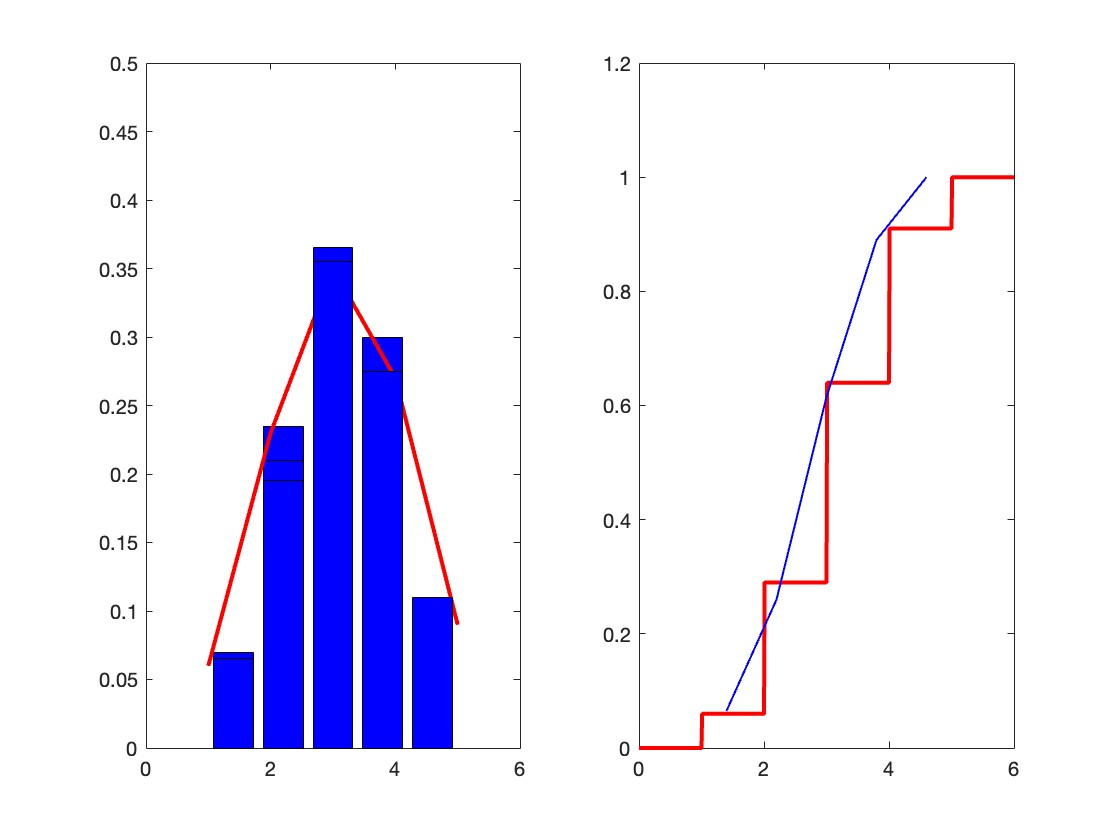
\includegraphics[width=0.8\linewidth]{../../assets/images/main-content-image.jpg}
    \caption{Kết quả mô phỏng kiểm định Pearson bằng MATLAB}
    \label{fig:pearson_test_result}
\end{figure}


\begin{matlab}
    \begin{lstlisting}
function Ngocppmohinh(c,j1,j2)
    %UNTITLED Summary of this function goes here
    % Version: 1.0
    %  Date: 10/09/24

    % So tham so
    numpara=j2-j1+1;
    % Dat cac tham so ban dau
    xmin=0; xmax=20; ymin=0; ymax=numpara*4;

    % Import the data
    singletons = readtable("singletons.xlsx");


    % Ve cac doi tuong thanh phan

    for i=1:numpara
    % Ve cac nut tren
    plot((xmin+xmax)/2,ymax-4*(i-1),'ob');
    hold on
    % Ve cac vi tri trang thai
        % tim vi tri cac hang trang thai cua tham so i
        hi=find([singletons{:,2}]==j1+i-1);
        % so trang thai thu i
        ni=length(hi);
        % so gia chia deu chieu ngang x
        dx=(xmax-xmin)/(ni+1);
        % vecto cac diem chia deu chieu ngang x
        x=xmin:dx:xmax;
        % Ve cac duong che ra
        % Vong lap cho tung trang thai
        for t=1:ni
        % Ve cac duong che ra
        plot([x(t+1) (xmin+xmax)/2],[ymax-4*(i-1)-2 ymax-4*(i-1)],'-r');
        hold on
        % Ve cac nut
        plot(x(t+1),ymax-4*(i-1)-2,'ob');
        hold on
        % Chen cac ten trang thai
        text(x(t+1)+.4,ymax-4*(i-1)-2-.4,singletons{hi(t),1});
        % Chen cac duong hoi tu
        plot([x(t+1) (xmin+xmax)/2],[ymax-4*(i-1)-2 ymax-4*(i-1)-4],'-r');
        hold on
        % Chen xac suat
        text(x(t+1)-.9, ymax-4*(i-1)-2+.4, [num2str(singletons{hi(t),5})]);
        end % t=1:ni
    end % for i=1:numpara

        % Ve nut ket thuc
        plot((xmin+xmax)/2,ymin,'ob');
        hold off
        
        % Chen cac 
        title('Graph of the clique Singletons')
        axis([xmin xmax ymin ymax+1])
        
        
        % Ve he truc hoac khong
        if c==0
            axis off
        else
            grid
        end % if c==0
        figure(1)

end % for function
    \end{lstlisting}
\end{matlab}

\begin{dl}
 Nội dung định lý viết vào đây   
\end{dl}

\cm{
Nội dung CM viết vào đây.
}

\begin{tc}
    
\end{tc}

\begin{md}
    
\end{md}

\begin{cy}
    
\end{cy}

\begin{vd}
    
\end{vd}

\begin{nx}
    
\end{nx}

\begin{bd}
    
\end{bd}
\subsection{Tiểu mục 2}
\begin{figure}[h!]
    \centering
    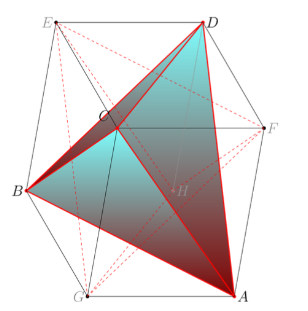
\includegraphics[width=0.6\linewidth]{../../assets/images/figure-1.png}
    \caption{Biểu đồ phân phối thống kê kiểm định}
    \label{fig:test_distribution}
\end{figure}
%%%%%%%%%%%%%%%%%%%%%%%%%%%%%%%%%%%%%%%%%%%%%%%%%%
% nội dung này có thể tham khảo giáo trình ĐSTT và HH2
\section{Mục 2}
\subsection{Tiểu mục 1}

\subsection{Tiểu mục 2}